\section{Formal results}
\label{sec:formal-results}

%\begin{itemize}
%	\item Results that we rely on (petri nets, semilinear sets)
%	\item The base algorithm described in math (without any optimizations)
%	\item Time complexity
%	\item proof for correctness of bidirectional pruning
%	\item mathematical description of optimizations
%\end{itemize}


\subsection{Background}

\paragraph{Petri Nets.}
A \emph{Petri net} is a tuple
\[
N = (P, T, \mathsf{pre}, \mathsf{post}, M_0),
\]
where \(P\) is a finite set of \emph{places}, \(T\) is a finite set of \emph{transitions},
\(\mathsf{pre},\mathsf{post}:T\to\mathbb N^P\) are the input/output vectors, and
\(M_0\in\mathbb N^P\) is the initial marking (token distribution). We use the terms \textit{state} and \textit{marking} interchangeably.

\noindent We say that a transition \(t\in T\) is \emph{enabled} at a marking \(M\in\mathbb N^P\) iff
\[
M \;\ge\; \mathsf{pre}(t)
\quad(\text{coordinate‐wise}).
\]
i.e., $M$ provides at least as many tokens as required by $\mathsf{pre}(t)$.
When $t$ is enabled at $M$, firing $t$ produces a new marking $M'$ defined as
\[
M' \;=\; M \;-\;\mathsf{pre}(t)\;+\;\mathsf{post}(t),
\]
which consumes input tokens and produces output tokens. We write $M \xrightarrow{t} M'$ when firing $t$ transforms $M$ to $M'$.
%
A marking \(M'\) is \emph{reachable} from $M$ via sequence $\sigma = t_1 \ldots t_k$ if there exist markings $M_0, \ldots, M_k$ where $M = M_0$, $M' = M_k$, and $M_i \xrightarrow{t_{i+1}} M_{i+1}$ for all $i$. We write $M \xrightarrow{\sigma} M'$.
%%
The set $R(N)$ contains all reachable markings:
\[
R(N) = \{M \mid \exists \sigma \in T^* .\ M_0 \;\xrightarrow{\sigma}\!^*\; M\}
\]
%
The \emph{reachability problem} asks, given a Petri net $N$ and a marking $M$, whether $M$ is reachable from $M_0$, the initial marking of $N$.  Surprisingly, even in the
\emph{unbounded} setting (where places may hold arbitrarily many tokens) this problem is
decidable~\cite{Ma81,Ko82,La92}, although with
Ackermann-complete complexity~\cite{CzWo22,Le22}.
%
An example of a toy Petri Net, and both reachable and unreachable markings, appears in Appendix~\ref{appendix:toyPN}.
%
%We focus on the verification of \textit{reachability properties}, meaning properties on the states that a net $N$ can reach. 
We check whether a marking satisfying formula $F$ (a combination of linear constraints) is reachable. The property is \textit{reachable} (\sat) if some $M \in R(N)$ satisfies $M \models F$, and \textit{unreachable} (\unsat) otherwise. 

\paragraph{Verdict proofs.} 

If a property $F$ is reachable in $N$, then a witness sequence $\sigma \in T^*$ and marking $M$ such that $ M_0 \;\xrightarrow{\sigma}\; M \text{ and }M \models F$
%\[
%M_0 \;\xrightarrow{\sigma}\; M \text{ and }M \models F
%\] 
serves as a proof of reachability. One can verify the claim by simulating $\sigma$ from $M_0$ and checking that the resulting marking satisfies $F$.
%
If $F$ is unreachable, there exists~\cite{Le09} an inductive certificate $C$ (a Presburger formula) satisfying:
(i) $M_0 \models C$ (initial state satisfies $C$);
(ii) if $M \models C$ and $M \xrightarrow{t} M'$, then $M' \models C$ (inductiveness); and
(iii) $C \Rightarrow \neg F$ (certificate implies property is false).

%
%\begin{enumerate}
%	\item $M_0 \models F$,
%	\item For all transitions $M \xrightarrow{t} M'$, if $M \models C$ then $M' \models C$,
%\item $C \Rightarrow \neg F$, i.e., all markings satisfying $C$ falsify $F$.
%\end{enumerate} 

\paragraph{Semilinear sets and Parikh’s theorem.}
A set \(S\subseteq\mathbb N^k\) is \emph{semilinear} iff
\[
S \;=\; \bigcup_{i=1}^m \Bigl\{\mathbf b_i + \sum_{j=1}^{r_i} n_j\,\mathbf p_{i,j}
\;\Big|\; n_j\in\mathbb N\Bigr\}.
\]

for $b_i, p_{i,j}\in \mathbb N^k$ being k-dimensional vectors of non-negative values.
%
Semilinear sets coincide exactly with the sets definable in \textit{Presburger arithmetic}~\cite{Pr29}.
%
By Parikh's theorem~\cite{Parikh66}, the \textit{Parikh Image} of any context-free language is semilinear, and there is an effective construction mapping each word in the language to a
finite description of its Parikh Image.

\paragraph{Deciding serializability in unbounded systems.}

We build on Bouajjani et al.~\cite{BoEmEnHa13}, who proved that serializability is decidable for unbounded systems by reducing it to Petri net reachability. They showed this as a special case of \textit{bounded-barrier linearizability}.



\subsection{The Algorithm (without Optimizations)}

Given a network system \(\mathcal S\) with global states \(G\), our algorithm proceeds as follows:  

\begin{enumerate}
	\item  \textbf{Serializability automaton.}  
	We define an NFA
	
\[
\mathcal A_{\mathrm{ser}}(\mathcal S)
= \bigl(Q,\Sigma,\delta,q_0,F\bigr),
\quad
Q = G
\quad\text{(the set of the NS’s global states)}
\]
\[
\Sigma
= \Bigl\{
{(\color{ForestGreen}\blacklozenge_{\mathit{req}}}\,/\,%
{\color{red}\blacklozenge_{\mathit{resp}}})
\;\Big|\;
{\color{ForestGreen}\blacklozenge_{\mathit{req}}}\in\mathit{REQ},\;
{\color{red}\blacklozenge_{\mathit{resp}}}\in\mathit{RESP}
\Bigr\}
\]
\[
\delta \;\subseteq\; Q \times \Sigma_{	{\color{ForestGreen}\blacklozenge_{\mathit{req}}}\,/\,%
	{\color{red}\blacklozenge_{\mathit{resp}}}} \times Q,
\quad
\bigl(q \xrightarrow{%
	{\color{ForestGreen}\blacklozenge_{\mathit{req}}}\,/\,%
	{\color{red}\blacklozenge_{\mathit{resp}}}%
} q'\bigr)
\;\Longleftrightarrow\;
\begin{array}{l}
	\mathcal S \text{ is in global state } q
	\;\text{and issues a request}\;
	{\color{ForestGreen}\blacklozenge_{\mathit{req}}},\\[0.5ex]
	\text{then upon completion it receives response}\;
	{\color{red}\blacklozenge_{\mathit{resp}}},\\[0.5ex]
	\text{and transitions to global state } q'
\end{array}
\]
%
%
%
%
%
%
%\begin{array}{l}
%	\mathcal S \text{ at global state } q
%	\;\text{issues}\;
%	{\color{ForestGreen}\blacklozenge_{\mathit{req}}},\\[0.5ex]
%	\text{after full completion of the request, it receives}\;
%	{\color{red}\blacklozenge_{\mathit{resp}}},\\[0.5ex]
%	\text{arriving at global state } q'
%\end{array}
%\]

	
	(i.e.\ each transition is a request/response pair).  Its language
	\(L(\mathcal A_{\mathrm{ser}})\subseteq\Sigma^*\) is exactly the set of serial
	request/response traces, and we define the semilinear set of serial executions, each such execution giving rise to a multiset of request/response pairs:
	\[
	\mathsf{Ser}(\mathcal S)
	\;=\;
	\mathsf{Parikh}\bigl(L(\mathcal A_{\mathrm{ser}})\bigr)
	\;\subseteq\;\mathbb N^{|\Sigma|}.
	\]
	
	\item 
	\textbf{Interleaving Petri Net.}
	
	We build
	\[
	N_{\mathrm{int}}(\mathcal S)
	= (P,\,T,\,\mathsf{pre},\,\mathsf{post},\,M_0),
	\]
	where
	\[
	P
	=
	P_G \;\cup\; P_{REQ,L} \;\cup\; P_{REQ,RESP}
	\]
	
	for 
	\[
	\begin{aligned}
		P_G
		&= \{\,p_g \mid g\in G\},\quad
		P_{REQ,L}
		= \bigl\{\,p_{({\color{ForestGreen}\blacklozenge_{\mathit{req}}}/\ell)}
		\mid {\color{ForestGreen}\blacklozenge_{\mathit{req}}}\in\mathit{REQ},\,\ell\in L\bigr\},\\[1ex]
		P_{REQ,RESP}
		&= \bigl\{\,p_{({\color{ForestGreen}\blacklozenge_{\mathit{req}}}/{\color{red}\blacklozenge_{\mathit{resp}}})}
		\mid {\color{ForestGreen}\blacklozenge_{\mathit{req}}}\in\mathit{REQ},\,
		{\color{red}\blacklozenge_{\mathit{resp}}}\in\mathit{RESP}\bigr\}.
	\end{aligned}
	\]
	
	
%	\[
%	\begin{aligned}
%		P_G &= \{\,p_g \mid g\in G\},\;\,
%		P_{REQ,L} = \{\,p_{{\color{ForestGreen}\blacklozenge_{\mathit{req}}}/\ell}
%		\mid {\color{ForestGreen}\blacklozenge_{\mathit{req}}}\in\mathit{REQ},\,\ell\in L\},\\
%		P_{REQ,RESP} &= \{\,p_{{\color{ForestGreen}\blacklozenge_{\mathit{req}}}/{\color{red}\blacklozenge_{\mathit{resp}}}}
%		\mid {\color{ForestGreen}\blacklozenge_{\mathit{req}}}\in\mathit{REQ},\,
%		{\color{red}\blacklozenge_{\mathit{resp}}}\in\mathit{RESP}\}.
%	\end{aligned}
%	\]
	
%	\[
%	P_G 
%	= \{\,p_g \mid g\in G\}
%	\quad 
%%	P_L 
%%	= \{\,p_\ell \mid \ell\in L\}
%%	\quad
%	P_{REQ,L} =
%	\{\,p_{{\color{ForestGreen}\blacklozenge_{\mathit{req}}}/\ell} \mid
%	{\color{ForestGreen}\blacklozenge_{\mathit{req}}}\in \mathit{REQ}, \ell\in L\},%\\
%	\quad
%	P_{REQ,RESP}=
%	\{\,p_{{\color{ForestGreen}\blacklozenge_{\mathit{req}}}/{\color{red}\blacklozenge_{\mathit{resp}}}} \mid
%	{\color{ForestGreen}\blacklozenge_{\mathit{req}}}\in \mathit{REQ}, {\color{red}\blacklozenge_{\mathit{resp}}}\in \mathit{RESP}\},
%	\]
%	\{\,p_{{\color{ForestGreen}\blacklozenge_{\mathit{req}}}/{\color{red}\blacklozenge_{\mathit{resp}}}} \mid
%	{\color{ForestGreen}\blacklozenge_{\mathit{req}}}\in \mathit{REQ}, {\color{red}\blacklozenge_{\mathit{resp}}}\in \mathit{RESP}\},
%	\]
	
%	\[
%	P_{REQ,RESP}=
%	\{\,p_{{\color{ForestGreen}\blacklozenge_{\mathit{req}}}/{\color{red}\blacklozenge_{\mathit{resp}}}} \mid
%	{\color{ForestGreen}\blacklozenge_{\mathit{req}}}\in \mathit{REQ}, {\color{red}\blacklozenge_{\mathit{resp}}}\in \mathit{RESP}\},
%	\]
	
	with \(G\) being the global states, \(L\) being the in‐flight local states (request‐state + remaining program), and \(\mathit{RESP}\) denoting the response labels.
	
	Transitions are partitioned as
	\[
	T = T_{\mathit{req}} \;\cup\; T_{\delta}\;\cup\;T_{\mathit{resp}}
	\]
	where
%	\[
%	T_{\mathit{req}} = \{\,t_{({\color{ForestGreen}\blacklozenge_{\mathit{req}}},\ell)} \mid {(\color{ForestGreen}\blacklozenge_{\mathit{req}}},\ell)\in\mathit{req}\},\quad
%	T_{\delta} = \{\,t_{(\ell,g)\to(\ell',g')} \mid (\ell,g)\xrightarrow{}(\ell',g')\in\delta\},\quad
%	T_{\mathit{resp}} = \{\,t_{(\ell,{\color{red}\blacklozenge_{\mathit{resp}}})} \mid (\ell,{\color{red}\blacklozenge_{\mathit{resp}}})\in\mathit{resp}\}.
%	\]
	
	\begin{align*}
		T_{\mathit{req}}
		&= \{\,t_{({\color{ForestGreen}\blacklozenge_{\mathit{req}}},\ell)} \mid {(\color{ForestGreen}\blacklozenge_{\mathit{req}}},\ell)\in\mathit{req}\},\\[1ex]
		T_{\delta}
		&= \bigl\{\,t_{(\ell,g)\to(\ell',g')} 
		\mid (\ell,g)\xrightarrow{}(\ell',g')\in\delta\bigr\},\quad
		T_{\mathit{resp}}
		= \{\,t_{(\ell,{\color{red}\blacklozenge_{\mathit{resp}}})} \mid (\ell,{\color{red}\blacklozenge_{\mathit{resp}}})\in\mathit{resp}\}.
	\end{align*}
	
	Their pre/post vectors are:
	\[
	\begin{alignedat}{3}
		\mathsf{pre}\bigl(t_{({\color{ForestGreen}\blacklozenge_{\mathit{req}}},\ell)}\bigr)
		&= \mathbf0, &
		\mathsf{post}\bigl(t_{({\color{ForestGreen}\blacklozenge_{\mathit{req}}},\ell)}\bigr)
		&= \mathbf1_{p_{({\color{ForestGreen}\blacklozenge_{\mathit{req}}},\ell)}}, 
		&&\text{for each }({\color{ForestGreen}\blacklozenge_{\mathit{req}}},\ell)\in\mathit{req},\\
		\mathsf{pre}\bigl(t_{(\ell,g)\to(\ell',g')}\bigr)
		&= \mathbf1_{p_{({\color{ForestGreen}\blacklozenge_{\mathit{req}}},\ell})} + \mathbf1_{p_g}, &
		\mathsf{post}\bigl(t_{(\ell,g)\to(\ell',g')}\bigr)
		&= \mathbf1_{p_{({\color{ForestGreen}\blacklozenge_{\mathit{req}}},\ell')}} + \mathbf1_{p_{g'}}, 
		&&\text{for each }(\ell,g)\!\to\!(\ell',g')\in\delta,\\
		\mathsf{pre}\bigl(t_{(\ell,{\color{red}\blacklozenge_{\mathit{resp}}})}\bigr)
		&= \mathbf1_{p_{({\color{ForestGreen}\blacklozenge_{\mathit{req}}},\ell)}}, &
		\mathsf{post}\bigl(t_{(\ell,{\color{red}\blacklozenge_{\mathit{resp}}})}\bigr)
		&= \mathbf1_{p_{({\color{ForestGreen}\blacklozenge_{\mathit{req}}}/{\color{red}\blacklozenge_{\mathit{resp}}})}}, 
		&&\text{for each }{{\color{ForestGreen}\blacklozenge_{\mathit{req}}}\in\mathit{req},(\ell,\color{red}\blacklozenge_{\mathit{resp}}})\in\mathit{resp}
		%\ %(\ell\text{ the matching local state).
%		}
	\end{alignedat}
	\]
	
	The initial marking is a single token on the place representing the initial global state $g_0$ of the NS:
	\[
	M_0(p_{g_0}) = 1,
	\quad
	M_0(p) = 0 \text{ for all }p\neq p_{g_0},
	\]
%	where \(g_0\) is the initial global state of the network system \(\mathcal S\).  
	
	
	
	Define the projection of all reachable markings to the places representing completed request/response pairs:
	\[
	\pi \;:\;\mathbb N^P \;\longrightarrow\;\mathbb N^{P_R}
	\quad\bigl(\pi(M)\bigr)(p_{({{\color{ForestGreen}\blacklozenge_{\mathit{req}}}/{\color{red}\blacklozenge_{\mathit{resp}}}})})\;=\;M(p_{({{\color{ForestGreen}\blacklozenge_{\mathit{req}}}/{\color{red}\blacklozenge_{\mathit{resp}}}})})\text{ for }p_{({{\color{ForestGreen}\blacklozenge_{\mathit{req}}}/{\color{red}\blacklozenge_{\mathit{resp}}}})}\in P_{REQ,RESP}.
	\]
	Then the multiset of all  (${{\color{ForestGreen}\blacklozenge_{\mathit{req}}}/{\color{red}\blacklozenge_{\mathit{resp}}}}$) pairs of the NS, attained by any interleaving, is:
	\[
	\mathsf{Int}(\mathcal S)
	\;=\;
	\bigl\{\;\pi(M)\;\bigm|\;M_0 \xrightarrow{}^{*} M\text{ in }N_{\mathrm{int}}(\mathcal S)\bigr\}.
	\]
	
	\item \textbf{Non-serializable set.}  
	Let
	\(\;\mathsf{NonSer}(\mathcal S)=\mathbb N^{|\Sigma|}\setminus \mathsf{Ser}(\mathcal S)\), i.e., all (${{\color{ForestGreen}\blacklozenge_{\mathit{req}}}/{\color{red}\blacklozenge_{\mathit{resp}}}}$) pairs that \textit{cannot} be attained via a serializable execution.
	
	\item \textbf{Reachability encoding.}  
	Ask whether there exists a marking \(M\) of \(N_{\mathrm{int}}(\mathcal S)\) such that
	\[
	M_0 \xrightarrow{}^{*} M
	\quad\wedge\quad
	\pi(M)\in \mathsf{NonSer}(\mathcal S).
	\]
	
	\item \textbf{Decision.}  
	\begin{itemize}
		\item [\sat]: yields a counterexample interleaving \(M\) with
		\(\pi(M)\notin \mathsf{Ser}(\mathcal S)\).
		\item [\unsat]: yields an inductive invariant of
		\(N_{\mathrm{int}}\), which back-translates to a proof of
		serializability for \(\mathcal S\).
	\end{itemize}



\item \textbf{Validation.}  

	\begin{itemize}
		
		\item[\sat]: We validate a reachable trace and embed it into the NS semantics, yielding a valid interleaving that produces request/response pairs unattainable under any serial execution.
		See the example in subsec.~\ref{subsec:ns-not-serializable}.
		
		\item[\unsat]: We synthesize an inductive invariant over the interleaving PN, thereby proving that the corresponding semilinear set cannot be realized by any interleaving.
		See the example in subsec.~\ref{subsec:ns-serializable}.
		
		
%	\item \sat: we validate the reachable trace and project it to the NS semantics to represent a valid interleaving that results into request/response pairs which cannot be attained in serial executions.
%	See example in subsec.~\ref{subsec:ns-not-serializable}.
	
%	\item \unsat:
%	we generate an inductive invariant over the interleaving PN, proving that the semilinear set cannot be attained via an interleaving.
%	See example in subsec.~\ref{subsec:ns-serializable}.
\end{itemize}

\end{enumerate}

\paragraph{Complexity Analysis.}
The core algorithm reduces serializability checking to Petri net reachability with semilinear target sets. 
Since the serial executions form a regular language (step 1), their Parikh Image is effectively semilinear by Parikh's theorem, with size exponential in the NFA.
The interleaving Petri net (step 2) has $O(|G| + |L| + |\mathit{REQ}| \times |\mathit{RESP}|)$ places and $O(|\mathit{REQ}| + |\delta| + |\mathit{RESP}|)$ transitions.
The reachability query (step 3) asks whether the Petri net can reach the complement of a semilinear set, which is decidable but Ackermann-complete~\cite{CzWo22}.
Without optimizations, even simple examples can generate Petri nets with hundreds of places and exponentially-sized semilinear constraints, making the approach impractical.
Our optimizations (Section~\ref{sec:optimizations}) dramatically reduce both the Petri net size and the semilinear set complexity.


%\guy{should we add/prove the following?}
%
%\begin{proposition}
%	Let $N_{\mathrm{int}}(\mathcal S)=(P,T,\mathsf{pre},\mathsf{post},M_0)$ be the interleaving Petri net constructed above, and let
%	\[
%	\pi\colon\mathbb N^P\to\mathbb N^{P_R}
%	\]
%	be the projection onto the request/response places $P_R$.  Then
%	\[
%	\mathsf{Int}(\mathcal S)
%	\;=\;
%	\{\;\pi(M)\;\mid\;M_0\xrightarrow{*}M\}.
%	\]
%\end{proposition}


\subsection{Example: Non-Serializable Program}
\label{subsec:ns-not-serializable}

\paragraph{Serializable NFA Extraction.}

Continuing the running (non-serializable) example presented in Listing~\ref{lst:MotivatingExample2NonSer}, the NS depicted in Fig.~\ref{fig:code2ExampleNS} allows us to also extract the NFA encoding all serial executions. The states encode the global variable values, and the edges encode request/response pairs for all serial executions. As can be seen in Fig.~\ref{fig:code2ExampleNFA}, serial executions can produce only request/response pairs of the type ({\color{ForestGreen}$\blacklozenge_\text{main}$/{\color{red}$\blacklozenge_1$}}). Furthermore, the only global state reachable in serial executions, when a request enters and exits the system, is [X=0].
%
Intuitively, this corresponds to the Listing~\ref{lst:MotivatingExample2NonSer} program updating [X:=1] as an intermediate assignment before yielding.

\begin{wrapfigure}{r}{0.50\textwidth}  % “r” = right, width = 0.5\textwidth
	\centering
	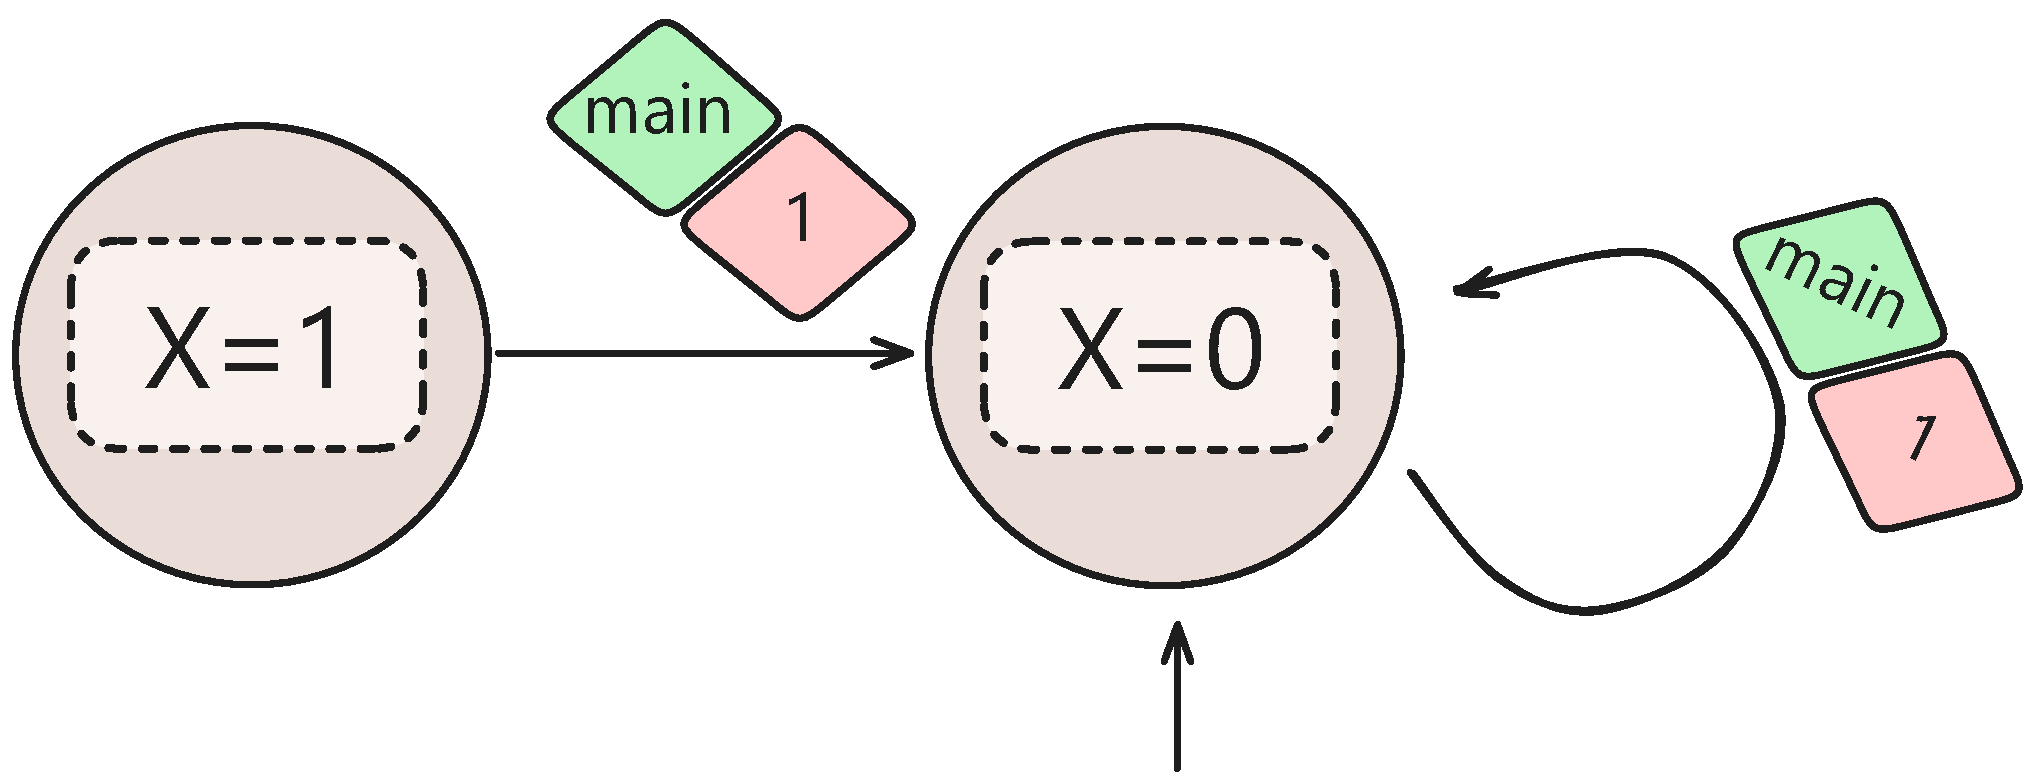
\includegraphics[width=0.48\textwidth,trim=0 0 0 0,clip]{plots/code_2_NFA_v3.pdf}
	\caption{Serial NFA of Listing~\ref{lst:MotivatingExample2NonSer}.}
	\label{fig:code2ExampleNFA}
\end{wrapfigure}


%\begin{wrapfigure}{r}{0.5\textwidth}  % “r” = right, width = 0.5\textwidth
%	\centering
%	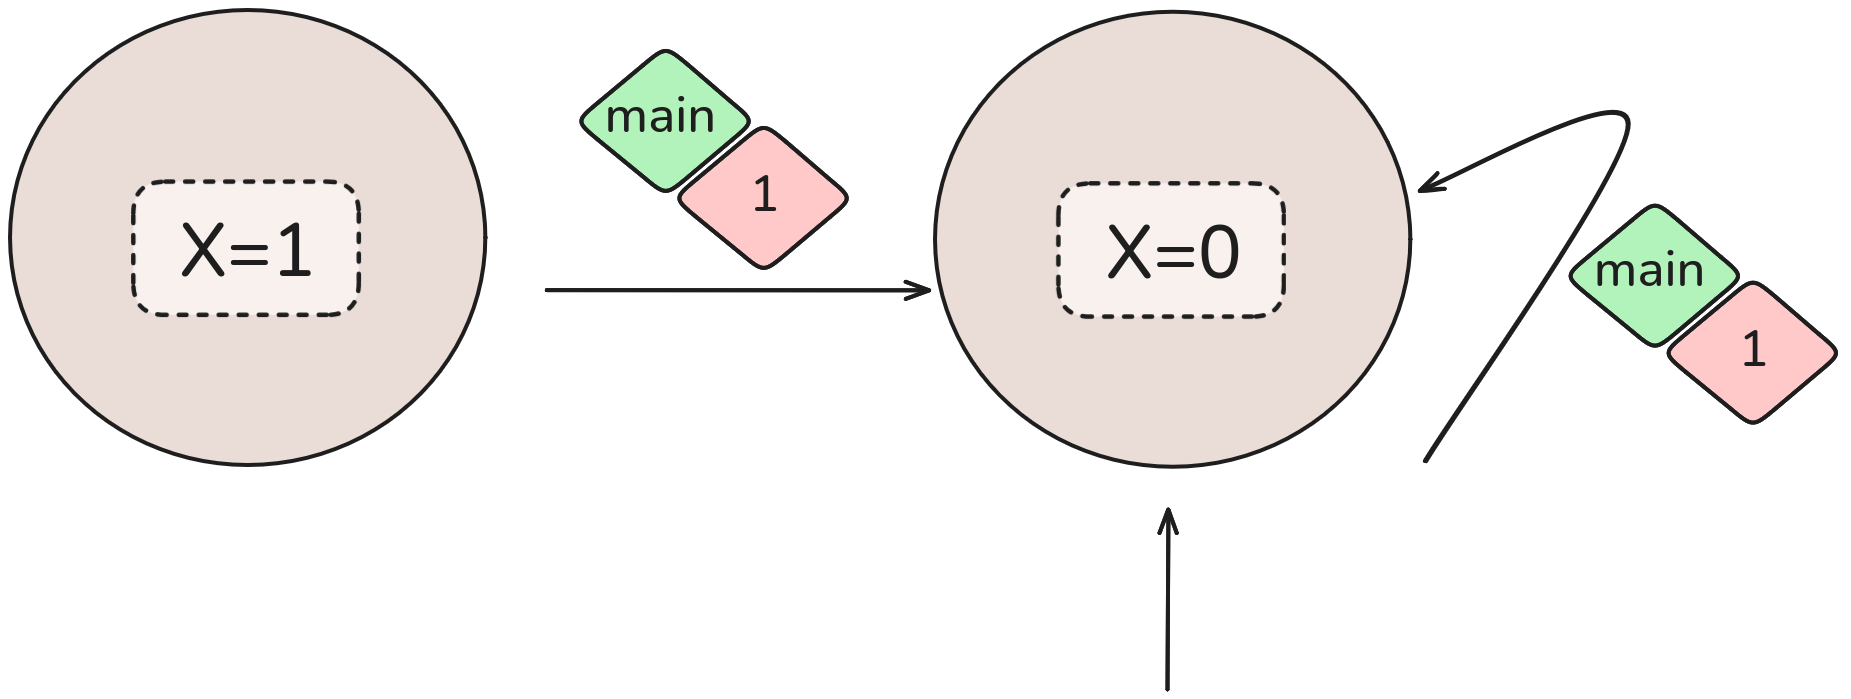
\includegraphics[width=0.48\textwidth,trim=0 0 0 0,clip]{plots/code_2_NFA.png}
%	\caption{NFA for serialized executions of Listing~\ref{lst:MotivatingExample2NonSer}.}
%	\label{fig:code2ExampleNFA}
%\end{wrapfigure}

%\begin{figure}[!htbp]
%	\centering
%	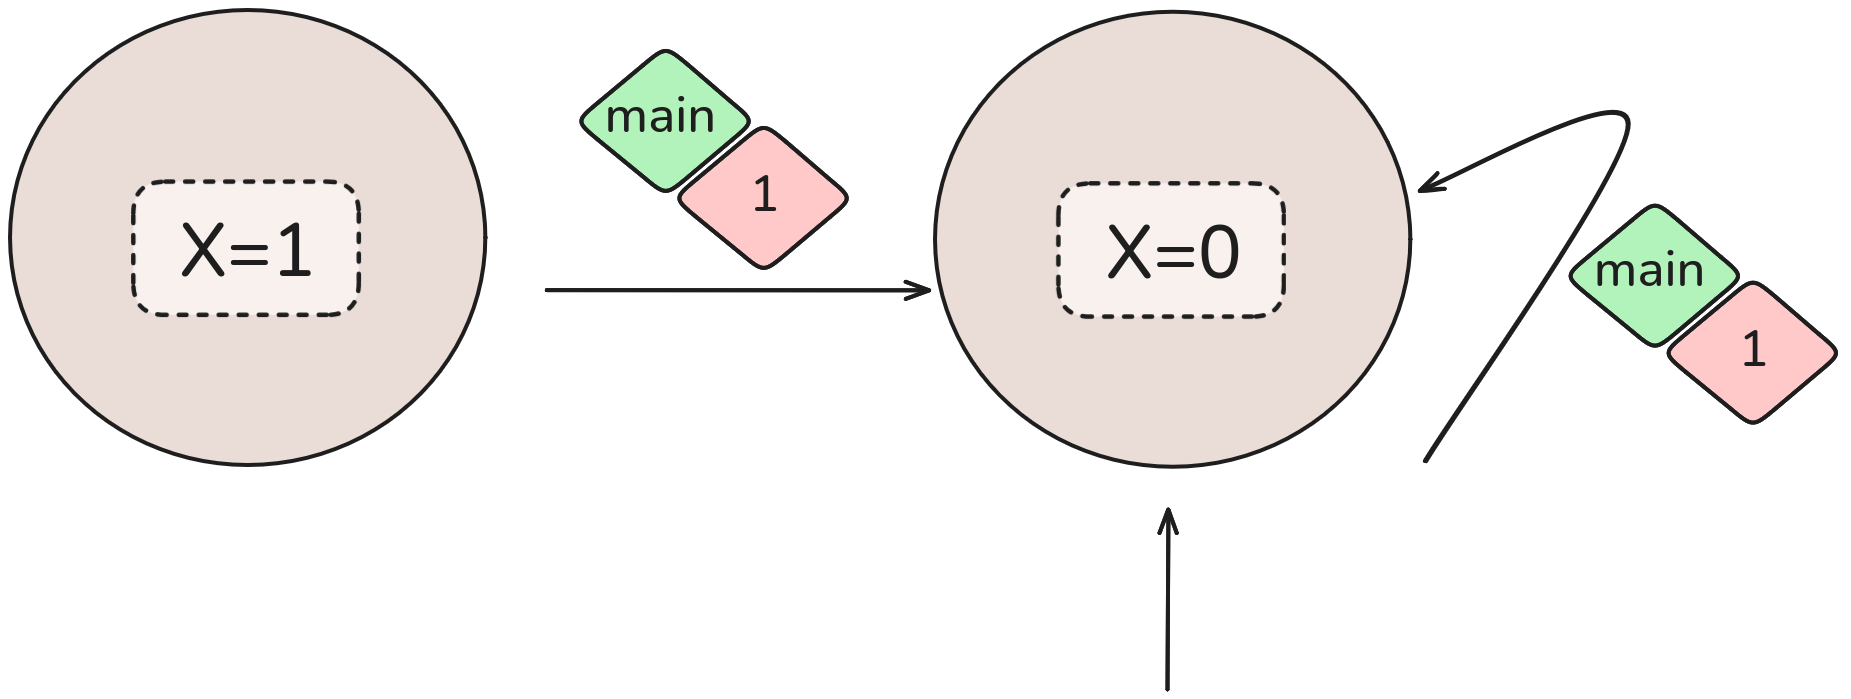
\includegraphics[width=0.5\textwidth,trim=0 0 0 0,clip]{plots/code_2_NFA.png}
%	\caption{NFA for serialized executions of Listing~\ref{lst:MotivatingExample2NonSer}.}
%	\label{fig:code2ExampleNFA}
%\end{figure}

\paragraph{Petri Net Extraction.}

Finally, the NS gives rise to the PN in Fig.~\ref{fig:code2ExamplePN}, encoding all possible interleavings. The places \textcolor{blue}{ $P_2$} and \textcolor{blue}{$P_3$} represent the global states \textcolor{blue}{[X=1]} and \textcolor{blue}{[X=0]}, respectively, while the places $P_1$, $P_4$, $P_5$, and $P_6$ capture the local states of in-flight requests—that is, the remaining program code together with the assignments to each request’s local variables. Similarly, places \textcolor{red}{$P_7$} and \textcolor{red}{$P_8$} correspond to {\color{red}$\blacklozenge_1$} and {\color{red}$\blacklozenge_0$}, respectively, encoding terminated responses. Each token either models an active request, a completed request/response pair, or --- when residing in a global-state place --- the current global state. Finally, transitions implement the network system’s mappings ($\delta/req/resp$): they advance the program by one step, spawn a new request (e.g., transition $t_1$, producing {\color{ForestGreen}$\blacklozenge_{\mathrm{main}}$}), or return a response (e.g., transitions $t_6$ and $t_7$).


%Finally, the NS gives rise to the PN in Fig.~\ref{fig:code2ExamplePN}, encoding all possible interleavings.
%%
%The places represent either the global state
%(e.g., places \textcolor{blue}{$P_2$} and \textcolor{blue}{$P_3$} correspond to the global states \textcolor{blue}{[X=1]} and \textcolor{blue}{[X=0]}), while others ($P_1,P_4,P_5,P_6$) correspond to the local state of an in-flight request, i.e., combinations of ``remaining'' programs  assignments to local variables of in-flight requests.
%%
%Furthermore, some requests correspond to responses, e.g., places \textcolor{red}{$P_7$} and \textcolor{red}{$P_8$} corresponds to {\color{red}$\blacklozenge_1$} and {\color{red}$\blacklozenge_0$}.
%%
%Each token corresponds either to a single in-flight request, a single terminated pair of request/response, or (in the case of the global-variable-encoding places), to the current global state.
%%
%Finally, transitions represent the network system's $\delta$ mapping --- encoding either a ``step'' of our program, or spawning a request ($t_1$, which  corresponds to spawning {\color{ForestGreen}$\blacklozenge_\text{main}$}), or returning a response (e.g. transitions $t_6,t_7$).
%


\begin{figure}[!htbp]
	\centering
	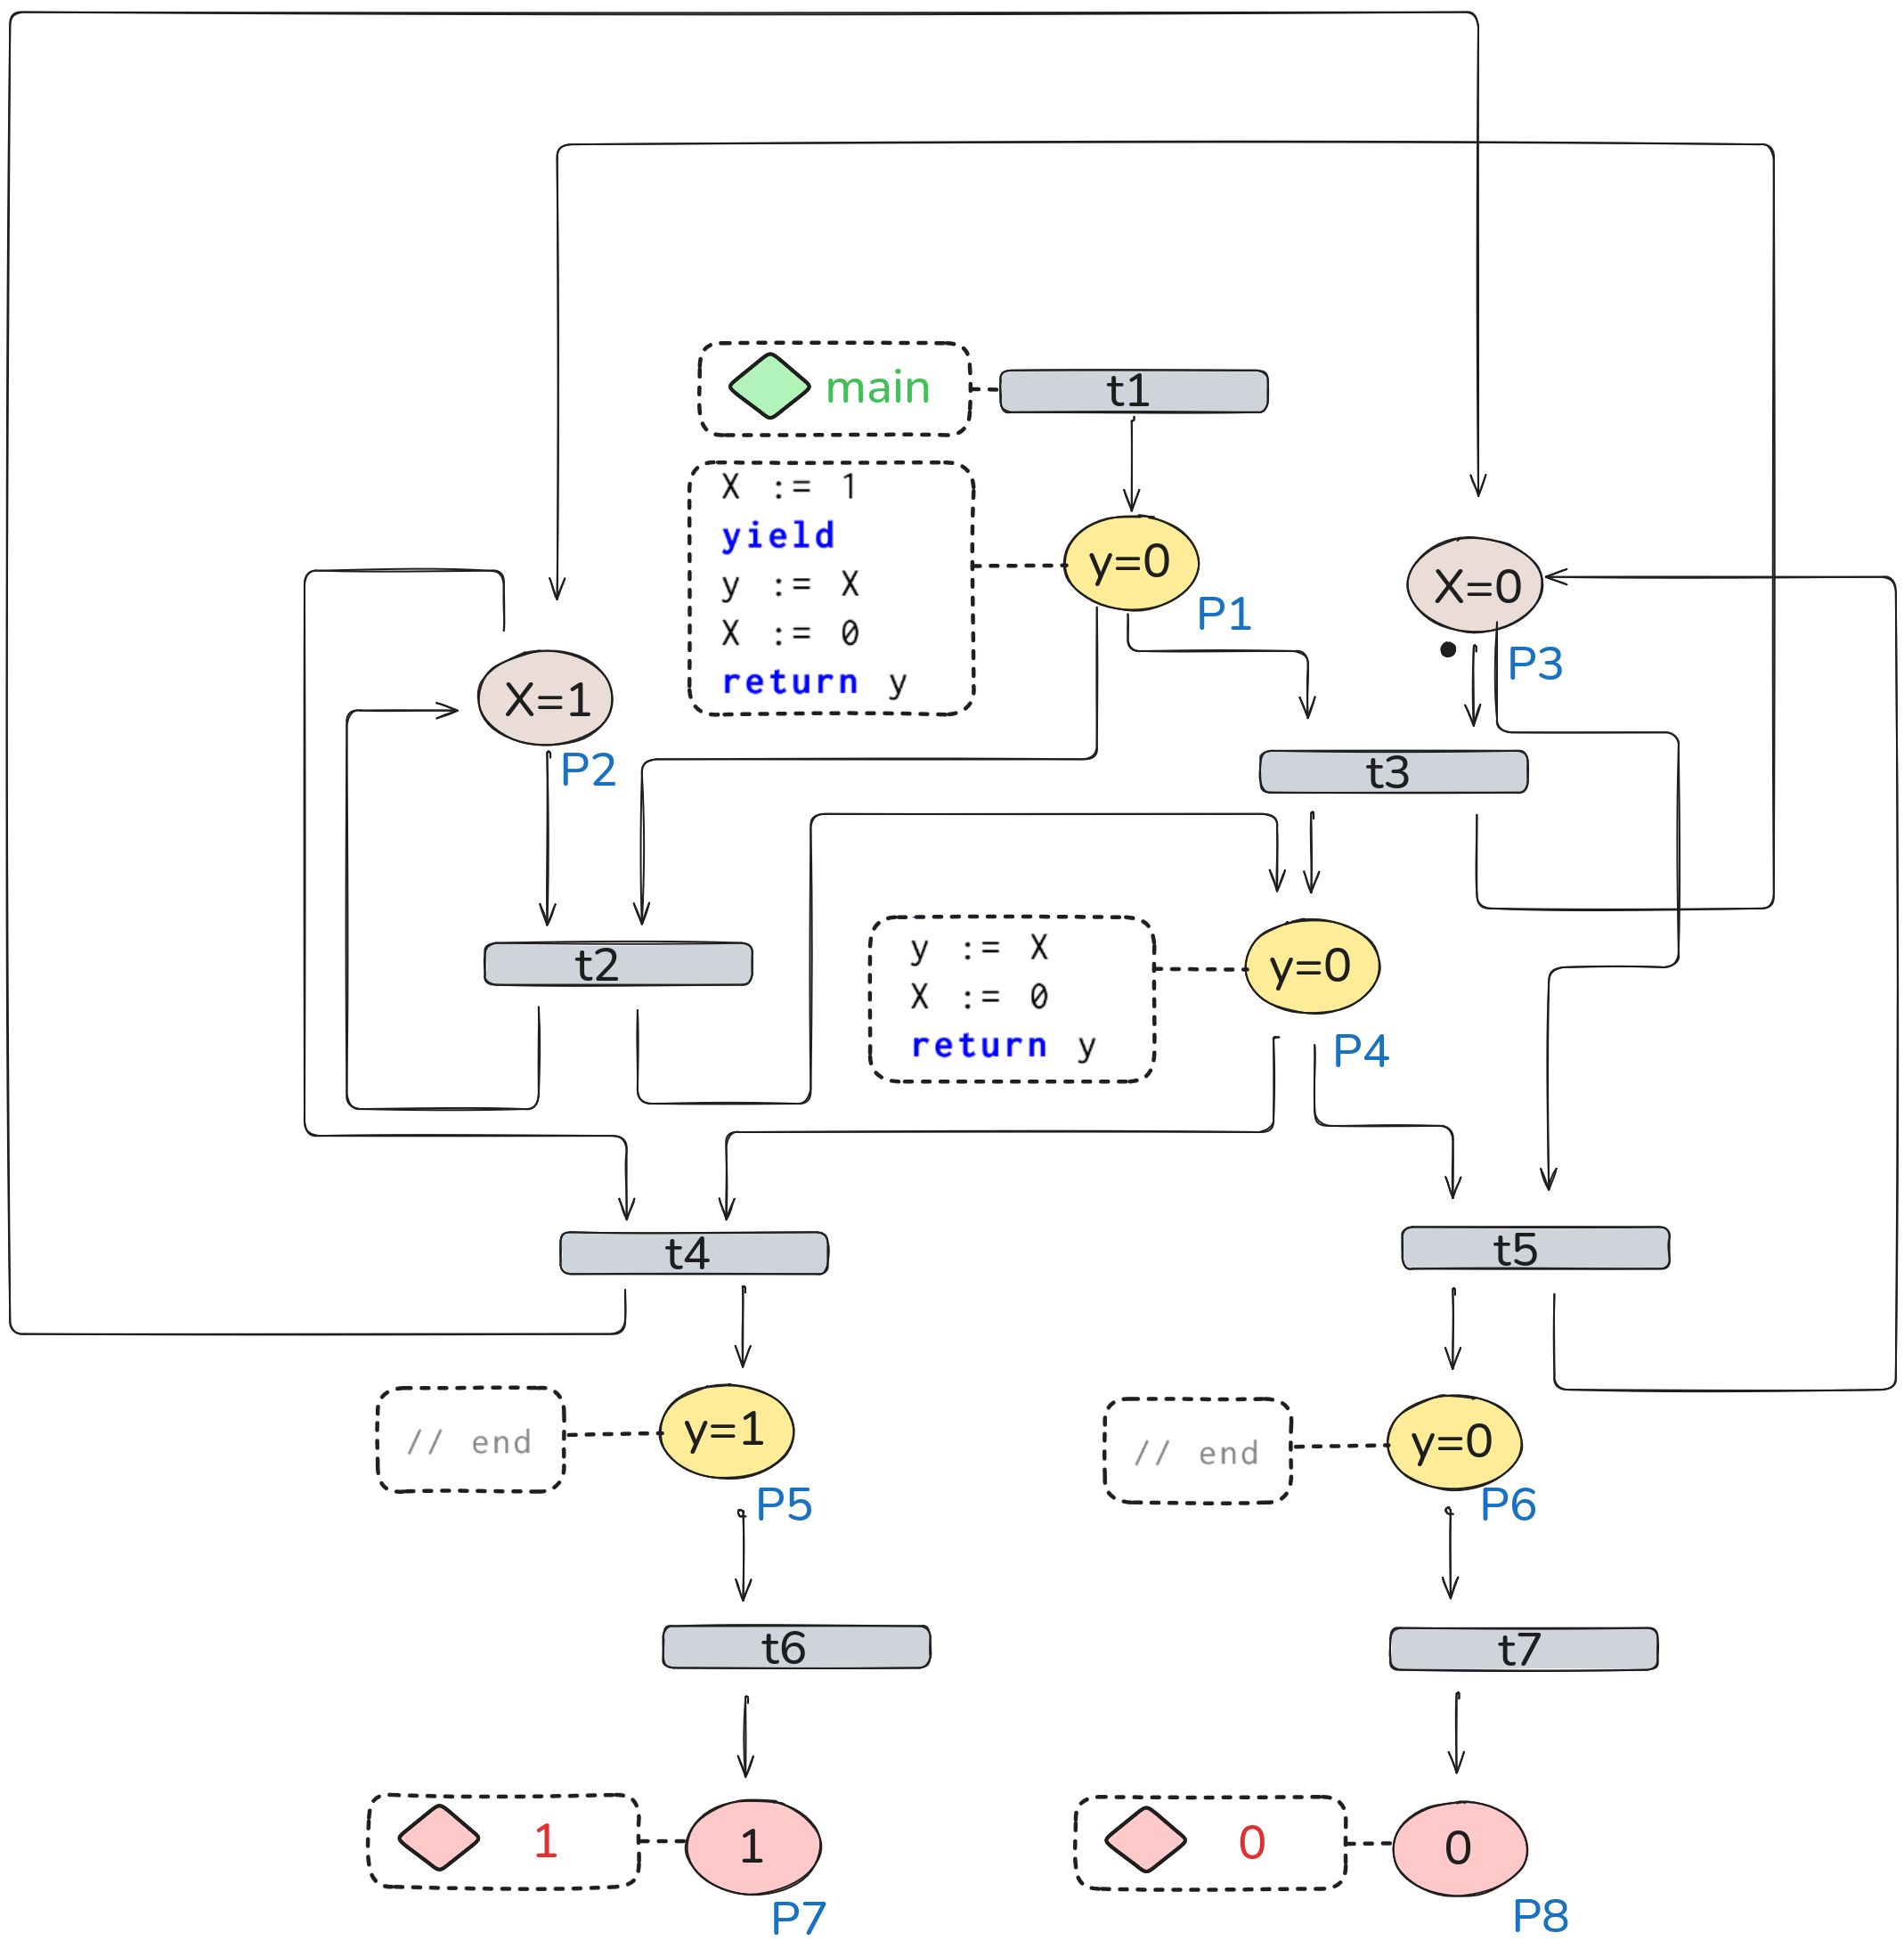
\includegraphics[width=0.7\textwidth]{plots/code_2_PN_with_annotation.png}
	\caption{The PN encoding interleaving executions of the program in Listing~\ref{lst:MotivatingExample2NonSer}.}
	\label{fig:code2ExamplePN}
\end{figure}

\paragraph{Counterexample Extraction.}

Regarding the aforementioned program, we automatically generate the following reachability query\footnote{If not for the equality constraints, the problem would have been considered a \textit{coverability} query, which is easier~\cite{Ra78}.} for the Petri net in Figure~\ref{fig:code2ExamplePN}: we encode the target semilinear set by imposing the following constraints on the token distribution:

%Regarding the aforementioned program, we automatically generate the following reachability query~\footnote{If not the equality constraints, the problem would have been considered a \textit{coverability} query which is easier~\cite{Ra78}.} for the Petri net in Figure~\ref{fig:code2ExamplePN} we encode a target semilinear set with the following constraints on the token distribution:
 

\[
P_1 = 0 \wedge 
\textcolor{blue}{P_2} \ge 0 \wedge \textcolor{blue}{P_3} \ge 0  \wedge P_4 = 0
\wedge P_5 = 0 \wedge P_6 = 0 \wedge \textcolor{red}{P_7} = 0 \wedge \textcolor{red}{P_8} \ge 1.
\]

This set encodes all reachable markings with no tokens on $P_1,P_4,P_5,P_6$,$\textcolor{red}{P_7}$, at least one token on $\textcolor{red}{P_8}$, and arbitrary tokens on $\textcolor{blue}{P_2},\textcolor{blue}{P_3}$.  
%
This target semilinear set of markings is, in fact non-empty. For example, it includes the following reachable marking:

\[
M^* = \{\textcolor{blue}{P_3}(1),\;\textcolor{red}{P_7}(1),\;\textcolor{red}{P_8}(1)\}
\]

Table~\ref{tab:PetriNetFiringCounterexample} lists a valid firing sequence that leads to $M^*$ from the initial state.
%
As the target set encodes request/response pairs that are \textit{unattainable} via serial executions, and as the PN encodes all possible interleavings, this firing sequence also corresponds as a counterexample demonstrating the program is non-serializable. 
%
As demonstrated by the outputs $\{{\color{ForestGreen}\blacklozenge_\text{main}}/{\color{red}\blacklozenge_0},{\color{ForestGreen}\blacklozenge_\text{main}}/{\color{red}\blacklozenge_1}\}$ (see Sec.~\ref{sec:introduction}).

\begin{table}[!htbp]
	\centering
	\label{tab:reach-seq}
	\begin{tabular}{c l c c c c c c}
		\toprule
		\textbf{Step} 
		& \textbf{Firing} 
		& \multicolumn{3}{c}{\textbf{Marking (after firing)}} 
		& \multicolumn{3}{c}{\textbf{Description (after firing)}} \\
		\cmidrule(lr){3-5} \cmidrule(lr){6-8}
		& 
		& \textbf{Global} 
		& \textbf{Local} 
		& \textbf{Responses} 
		& \textbf{Global state} 
		& \textbf{In-flight requests} 
		& \textbf{Responses} \\
		\midrule
		0 & --                                  
		& {\color{blue}$P_3$(1)}                  
		& --                                    
		& --                                    
		& {\color{blue}[X=0]}                   
		& --                          
		& --                                    \\
		1 & $t_1$ 
		& {\color{blue}$P_3$(1)}                  
		& $P_1$(1)                                
		& --                                    
		& {\color{blue}[X=0]}                   
		& {\color{ForestGreen}$\blacklozenge_\text{main}$} 
		& --                                    \\
		2 & $t_1$ 
		& {\color{blue}$P_3$(1)}                  
		& $P_1$(2)                                
		& --                                    
		& {\color{blue}[X=0]}                   
		& {\color{ForestGreen}$\blacklozenge_\text{main}$}, {\color{ForestGreen}$\blacklozenge_\text{main}$}  
		& --                                    \\
		3 & $t_3$                                  
		& {\color{blue}$P_2$(1)}                  
		& $P_1$(1),$P_4$(1)                          
		& --                                   
		&                                    {\color{blue}[X=1]}    
		&                                    {\color{black}$\blacklozenge_\text{until yield}$}, {\color{ForestGreen}$\blacklozenge_\text{main}$}   
		& --                                    \\
		4 & $t_2$                                  
		& {\color{blue}$P_2$(1)}                  
		& $P_4$(2)                                
		& --                                    
		&                                    {\color{blue}[X=1]}    
		&                                    {\color{black}$\blacklozenge_\text{until yield}$}, {\color{black}$\blacklozenge_\text{until yield}$}   
		& --                                    \\
		5 & $t_4$                                  
		& {\color{blue}$P_3$(1)}                  
		& $P_5$(1),$P_4$(1)                          
		& --                                    
		&                                   {\color{blue}[X=0]}     
		&                                    {\color{black}$\blacklozenge_\text{after yield}$}, {\color{black}$\blacklozenge_\text{until yield}$}   
		& --                                    \\
		6 & $t_6$                     
		& {\color{blue}$P_3$(1)}                  
		& $P_4$(1)                                
		& {\color{red}$P_7$(1)}                    
		&                                      	{\color{blue}[X=0]}  
		&                                    {\color{black}$\blacklozenge_\text{until yield}$}   
		&                                   {\color{red}$\blacklozenge_1$}     \\
		7 & $t_5$                                  
		& {\color{blue}$P_3$(1)}                  
		& $P_6$(1)                                
		& {\color{red}$P_7$(1)}                    
		&                                   {\color{blue}[X=0]}    
		&                                    {\color{black}$\blacklozenge_\text{after yield}$}      
		&                                   {\color{red}$\blacklozenge_1$}        \\
		8 & $t_7$                     
		& {\color{blue}$P_3$(1)}                                  
		& --                                    
		& {\color{red}$P_7$(1),\color{red}$P_8$(1)}    
		&                                   {\color{blue}[X=0]}    
		&                                   --    
		&                                   {\color{red}$\blacklozenge_0$}, {\color{red}$\blacklozenge_1$}       \\
		\bottomrule
	\end{tabular}
	\caption{The firing sequence reaching marking $M^*$ which is in our target semilinear set. The marking $P_i(n_j)$ indicates that there are $n_j$ tokens on place $P_i$. The initial marking has a single token in place $P_3$ encoding $g_0$.}
	\label{tab:PetriNetFiringCounterexample}
\end{table}

%\newpage

\subsection{Example: Serializable Program}
\label{subsec:ns-serializable}

Now, we observe again the adjusted program with locks (as previously described in Listing~\ref{lst:MotivatingExample3Ser}).
%
Due to space limitations, we relegate figures of the corresponding network system (Fig.~\ref{fig:code3ExampleNS}), Serializability NFA (Fig.~\ref{fig:code3ExampleNFA}), and Interleaving Petri Net (Fig.~\ref{fig:code3ExamplePN}) to Appendix~\ref{appendix:MoreNsExamples}, and focus on the serializability proof certificate.
%
In this specific example, non-serializability corresponds to the Petri Net being able to reach a marking satisfying the same semilinear formula as in the previous example for non-serializability (note however, that this is not always the case). 
%(but this time each place $P_i$ corresponds to the new PN). 
%following formula:
%
%\[
%\textcolor{blue}
%P_1 = 0 \wedge 
%{P_2} \ge 0 \wedge \textcolor{blue}{P_3} \ge 0  \wedge P_4 = 0
%\wedge P_5 = 0 \wedge P_6 = 0 \wedge \textcolor{red}{P_7} = 0 \wedge \textcolor{red}{P_8} \ge 1.
%\]


In addition, although the target set is the same as in the previous example, however, the Petri Net places $(P_1,\ldots,P_8)$ encode different states that correspond to the updated program. For example, now each place in the PN that encodes a global state accounts for two global variables, $X$ and $L$, and the initial global state corresponds to the place encoding the initial assignment \textcolor{blue}{[X=0, L=0]}, etc.
%
Furthermore, unlike the previous example, this target set of markings (encoding request/response pairs of non-serial executions) is \textit{unreachable}, as witnessed by the inductive invariant:


\[
\begin{aligned}
	&(P_{1},\textcolor{blue}{P_{2}},\textcolor{blue}{P_{3}},P_{4},P_{5},P_{6},\textcolor{red}{P_{7}},\textcolor{red}{P_{8}})
	\;\mapsto\;\\
	&\quad
	\exists\,e_{0},\dots,e_{5}\ge0.\;
	\Bigl(
	e_{2}-e_{1}+\textcolor{blue}{P_{3}}-1=0\;\land\;
	e_{2}+P_{1}-e_{5}=0\;\land\;
	P_{5}-e_{1}+e_{4}=0\;\land\\
	&\qquad\quad
	-\,e_{4}+\textcolor{red}{P_{7}}=0\;\land\;
	P_{6}+e_{3}-e_{0}=0\;\land\;
	\textcolor{red}{P_{8}}-e_{3}=0\;\land\\
	&\qquad\quad
	-\,e_{2}+e_{1}+e_{0}+P_{4}=0\;\land\;
	-\,e_{2}+e_{1}+\textcolor{blue}{P_{2}}=0
	\Bigr)
	\;\land\;
	\bigl(P_{4}-1\ge0\;\lor\;\textcolor{blue}{P_{3}}-1\ge0\bigr).
\end{aligned}
\]


We then revert and project it on request/response pairs of the network system.
%
We get the following inductive invariants for each of the two (reachable) global states:

\begin{proof}
	
	\medskip\noindent
	For global state \textcolor{blue}{[L=0,X=0]}
	the projected invariant is:
	\[
	\bigl(\,\text{\color{ForestGreen}$\blacklozenge_{\text{main}}$}/\text{\color{red}$\blacklozenge_{0}$},\;
	\text{\color{ForestGreen}$\blacklozenge_{\text{main}}$}/\text{\color{red}$\blacklozenge_{1}$}\bigr)
	\;\mapsto\;
	\exists\,e_{0},\dots,e_{5}\ge0.\;
	\begin{aligned}[t]
		& e_{2}-e_{1}=0,\quad
		e_{2}-e_{5}=0,\quad
		-e_{1}+e_{4}=0,\\
		& -e_{4}+\bigl(\text{\color{ForestGreen}$\blacklozenge_{\text{main}}$}/\text{\color{red}$\blacklozenge_{1}$}\bigr)=0,\quad
		-e_{0}+e_{3}=0,\quad
		-e_{3}+\bigl(\text{\color{ForestGreen}$\blacklozenge_{\text{main}}$}/\text{\color{red}$\blacklozenge_{0}$}\bigr)=0,\\
		& -e_{2}+e_{1}+e_{0}=0,\quad
		-e_{2}+e_{1}=0.
	\end{aligned}
	\]
	From these:
	\[
	e_{1}=e_{2}=e_{4}=e_{5}=(\;
	\text{\color{ForestGreen}$\blacklozenge_{\text{main}}$}/\text{\color{red}$\blacklozenge_{1}$}),\;
	e_{0}=e_{3}=
	(\text{\color{ForestGreen}$\blacklozenge_{\text{main}}$}/\text{\color{red}$\blacklozenge_{0}$}),
	\]
	and
	\[
	-e_{2}+e_{1}+e_{0}=0\;\Longrightarrow\;e_{0}=0.
	\]
	Thus
	\[
	(	\text{\color{ForestGreen}$\blacklozenge_{\text{main}}$}/\text{\color{red}$\blacklozenge_{0}$})
	=0,
	\]
	indicating that  (\(\text{\color{ForestGreen}$\blacklozenge_{\text{main}}$}/\text{\color{red}$\blacklozenge_{0}$}\)) cannot be attained from the global state
	\textcolor{blue}{[L=0,X=0]}.
	
	\medskip\noindent
	In the second case, for the global state \textcolor{blue}{[L=1, X=1]}
	the projected invariant is:
	
	
	\[
	\bigl(\,\text{\color{ForestGreen}$\blacklozenge_{\text{main}}$}/\text{\color{red}$\blacklozenge_{0}$},\;
	\text{\color{ForestGreen}$\blacklozenge_{\text{main}}$}/\text{\color{red}$\blacklozenge_{1}$}\bigr)
	\;\mapsto\;
	\exists\,e_{0},\dots,e_{5}.\;\bot,
	\]
	which is unsatisfiable. Hence, no completed request/response pair, and in particular no (\(\text{\color{ForestGreen}$\blacklozenge_{\text{main}}$}/\text{\color{red}$\blacklozenge_{0}$}\)) can be produced from this state via \textit{any} execution. Intuitively, this aligns with the fact that there cannot be any output generated via an interleaving, given that the lock is acquired (\textcolor{blue}{[L=1]}) 
	\guy{Mark/Jules is this part correct?}
	
	\medskip
	\noindent\textbf{Conclusion.}
	In every reachable state, no request/response pair of the form
	($	\text{\color{ForestGreen}$\blacklozenge_{\text{main}}$}/\text{\color{red}$\blacklozenge_{0}$})
	$
	can occur. Consequently, the only possible pairs are
	($	\text{\color{ForestGreen}$\blacklozenge_{\text{main}}$}/\text{\color{red}$\blacklozenge_{1}$})
	$,
	all of which lie within the NFA’s language for serial executions.
	Hence, the program is serializable. Moreover, as proven in Appendix~\ref{appendix:InductiveInvariantExample},
	these invariants are inductive: they hold in the initial state and are preserved under every transition.
\end{proof}
	
%	\medskip\noindent
%	\textbf{Conclusion.}
%	In all reachable states
%	it holds that there cannot be any request/response pair of type
%	(	$	\text{\color{ForestGreen}$\blacklozenge_{\text{main}}$}/\text{\color{red}$\blacklozenge_{0}$}
%	$).
%	%
%	Furthermore, this indicates that the only attainable request/response pairs are of the form 	($	\text{\color{ForestGreen}$\blacklozenge_{\text{main}}$}/\text{\color{red}$\blacklozenge_{1}$})
%	$, which are included in the language of of NFA for serial executions. Thus, this program is serializable.
%	%
%	We further show (in Appendix~\ref{appendix:InductiveInvariantExample}) that these invariants are \textit{inductive}: they encompass the system’s initial state and, once satisfied, remain true for all subsequent executions.




%\newpage


\subsection{Time/Space Complexity}

\guy{Should we add something about time/space complexity?}


\subsection{Optimizations}
\label{sec:optimizations}

%\todo{check}

We apply four optimizations to the base algorithm to control intermediate blow‐up in the size of both the PN and the constructed semilinear set. 
%
An extensive empirical evaluation of these optimizations appears later on in subsec.~\ref{subsec:optimization-results}.

\paragraph{(1) Bidirectional Petri net pruning.}  
This optimization concerns the very last step of the algorithm: solving the Petri net reachability problem.
For a given Petri net reachability problem, it may be that only some of the places and transitions are relevant.
So before any heavy symbolic reasoning takes place, we identify places that are necessarily always empty on any potential path from the start state to an end state, and remove them from the Petri net.

Formally, let $N=(P,T,\Pre,\Post,M_0)$ be a Petri net, and $S\subseteq\mathbb{N}^P$ a target set. By convention, we assume that $P$ and $T$ are disjoint.

\begin{definition}[Forward Over-Approximation]
	Define the operator $\mathcal{F}:\mathcal{P}(P\cup T)\to\mathcal{P}(P\cup T)$ by
	\[
	X \mapsto X
	~\cup~
	\{\,t\in T \mid \forall p\in P:\; \Pre(p,t)>0 \implies p\in X\}
	~\cup~
	\{\,p\in P \mid \exists t\in X\cap T,\ \Post(p,t)>0\}.
	\]
	Starting from $X_0 = \{\,p\mid M_0(p)>0\}$, iterate
	$X_{i+1} = \mathcal{F}(X_i)$ until a least fixed-point
        $X^*=\bigcup_i X_i$ is reached.  Call $X^*\cap P$ (resp. $X^* \cap T$) the set of
        \emph{forward-reachable} places (resp. transitions).
\end{definition}

\begin{definition}[Backward Over-Approximation]
	Let
	\[
	Y_0 = \{\,p\in P \mid \exists M\in S:\;M(p)\neq0\}
	\]
	be the places unconstrained to zero by the target.  Define
	$\mathcal{B}:\mathcal{P}(P\cup T)\to\mathcal{P}(P\cup T)$ by
	\[
	Y \mapsto Y
	~\cup~
	\{\,t\in T \mid \forall p\in P:\; \Post(p,t)>0 \implies p\in Y\}
	~\cup~
	\{\,p\in P \mid \exists t\in Y\cap T,\ \Pre(p,t)>0\}.
	\]
	Iterate $Y_{i+1} = \mathcal{B}(Y_i)$ until a least fixed-point
        $Y^*=\bigcup_i Y_i$ is reached.  Call $Y^*\cap P$ (resp. $Y^* \cap T$) the set of
        \emph{backward-relevant} places (resp. transitions).
\end{definition}

In the forward pass, we traverse from the initial marking to identify an over-approximation of all places and transitions that could ever fire; symmetrically, in the backward pass, we traverse backward from any place that can influence a target constraint, and identify an over-approximation of the places and transitions which may fire along a transition sequence ending at an end state.
In bidirectional pruning, we iteratively remove non-forwards-reachable and
non-backwards-relevant places and transitions, to a fixed point.
% This pruning can be quite effective: in the best
% case, we can discover that the target set is not reachable without needing to
% invoke the solver.

\begin{theorem}[Bidirectional Pruning Soundness]
\label{thm:bidirectional-pruning}
  Let $N = (P, T, \mathsf{pre}, \mathsf{post}, M_0)$ be a Petri net and $S$ a target set of markings.
  %
  Let $P^\ast, T^\ast$ be the fixed point of the bidirectional pruning algorithm and $N' = (P^*, T^*, \Pre|_{P^*,T^*}, \mathsf{post}|_{T^*}, M_0)$ be the pruned net.

  Then $S$ is reachable from $N$ iff it is reachable from $N'$.
\end{theorem}
%
We depict this in Fig.~\ref{fig:bidirectional_pruning}, and prove Theorem~\ref{thm:bidirectional-pruning} in Appendix~\ref{appendix:BidirectionalProof}.
% (see the proof in Appendix~\ref{appendix:BidirectionalProof}).
%

% \medskip
% \noindent\textit{\textbf{Intuition.}}
% Before any heavy symbolic reasoning takes place, we apply bidirectional pruning on the underlying PN.  In the forward pass, we traverse from the initial marking to identify an over-approximation of all places and transitions that could ever fire; in the backward pass, we traverse backward from any place that can influence a target constraint, and identify over-approximations on transitions and places that cannot contribute to reaching it.  By iteratively repeating forward passes and backward passes until convergence, we remove every component of the net that cannot both originate and contribute to the reachable target set.  This dramatically shrinks the net in practice, often converting an intractably large model into one small enough for exhaustive analysis.


\paragraph{(2) Semilinear set pruning.}  
Recall that a semilinear set is $S=\bigcup_{i=1}^m L_i$, with
\[
\displaystyle L_i=\{\,b_i+\sum_{p\in P_i}n_p p\mid n_p\in\mathbb N\}.
\]
When manipulating semilinear sets, we may end up with redundant representations:
redundant period vectors $p \in P_i$ or even whole redundant components $L_i$.

We prune semilinear sets while building them to remove such redundancies.
\begin{itemize}
  \item For each $P_i$, we greedily remove any $p \in P_i$ which is already a
    nonnegative linear combination of $P_i \setminus \{p\}$.
  \item Whenever $L_i \subseteq L_j$ for $i \neq j$, we remove the redundant $L_i$.
\end{itemize}

Keeping semilinear sets small reduces prevents unecessary blow-ups in the size of the formulas that get passed to solvers, which is important to keep solver invocations tractable.

% it is common for some inequalities or disjuncts to add no new coverage beyond what other constraints already guarantee.  The redundant‐constraint elimination pass inspects each linear inequality and each disjunct in a disjunctive normal form, testing whether it is implied by the rest.  Any constraint or disjunct found redundant is dropped, ensuring that subsequent intersection, union, and projection operations work on the smallest necessary formula.  This streamlines the logic formula and prevents unnecessary size blow‐ups during solver invocations.

% %
% We replace each period‐basis \(P_i\) by
% \[
% P_i \;:=\;\{\,p\in P_i \mid p\notin\mathsf{Span}(P_i\setminus\{p\})\}
% \],
% Dropping any ``redundant'' periods, and removing any \(L_j\subseteq L_i\) for \(i\neq j\), iterating to a fixed point so no two components subsume one another.

\paragraph{(3) Generating fewer constraints.}
When computing the Parikh image of a regular expression as a semilinear set,
most regex operations can be implemented without exponential blow-up.
However, Kleene star is a notable exception: in the general case, the
semilinear set $S^\ast$ has an exponentially larger representation than $S$
itself.  Therefore, we implement optimizations specifically to reduce the size
of $S^\ast$ when possible.

Let $S$ be the semilinear set $\bigcup_{i=1}^m L_i$, with
\[
  L_i=\left\{\,b_i+\sum_{p\in P_i}n_p p \mid n_p\in\mathbb N \right\},
\]
as above. In the general case, the Kleene star $S^\ast$ is given as a semilinear set by
\[
  \bigcup_{I \subseteq \{1,...,m\}} \left\{
    \sum_{i \in I} b_i
    + \sum_{p \in \bigcup_{i \in I} P_i} n_p p \mid n_p \in \mathbb N \right\}.
\]
As the index set $I$ runs over all subsets of $\{1,...,m\}$, this has $2^m$ many components. However, in a typical case, we may not need that many. We implement the following special-case optimizations:
\begin{itemize}
  \item If any component $L_i$ of $S$ has no period vectors, $L_i = \{b_i\}$, then we can pull it out separately, computing the Kleene star of the rest and then adding $b_i$ as a period vector to every linear component of the result.

  \item Likewise, if any component $L_i$ of $S$ has a zero \emph{base} vector,
    $L_i = \{ \sum_{p \in P_i} n_p p \mid n_p \in \mathbb N\}$,
    we can pull it out separately, computing the Kleene star of the rest and adding each $p \in P_i$ as a period vector to every linear component of the result.
\end{itemize}
Each reduces the number of components generated from a Kleene star by
half, whenever it applies.

% Let $\mathrm{comp}(S)=\{L_1,\dots,L_m\}$ 
% be the multiset of linear components of the semilinear set 
% \(\displaystyle S=\bigcup_{i=1}^m L_i\), where each 
% \(\;L_i=b_i+\langle P_i\rangle\) with \(b_i\in\mathbb N^d\) and 
% \(P_i\subseteq\mathbb N^d\).  Define the pruning operator
% \[
% \mathrm{new}(\mathcal C)
% \;=\;
% \bigcup\bigl\{\,L\in\mathcal C \;\bigm|\;\nexists\,L'\in\mathcal C\setminus\{L\}:\;L'\subsetneq L\bigr\},
% \]
% which removes any component strictly containing another.  
% %
% \guy{Nicolas is it clear we mean that we fix their semilinear "meaning" of the regex operations? For example, + is union etc..}
% Then, we replace the naive semilinear‐set operations by
% \[
% S\;+\;T
% \;=\;
% \mathrm{new}\bigl(\mathrm{comp}(S)\,\cup\,\mathrm{comp}(T)\bigr),
% \]
% \[
% S\;\cdot\;T
% \;=\;
% \mathrm{new}\Bigl(\{\,L_i\cdot L'_j \mid L_i\in\mathrm{comp}(S),\;L'_j\in\mathrm{comp}(T)\}\Bigr),
% \]
% where for
% \(\;L_i=b_i+\langle P_i\rangle,\;L'_j=b'_j+\langle P'_j\rangle\) we set
% $
% L_i\cdot L'_j
% =\;(b_i+b'_j)\;+\;\langle\,P_i\cup P'_j\,\rangle.
% $
% Finally, for Kleene‐star and plus on the regex side one similarly applies
% \(\mathrm{new}(\cdot)\) to the collection of ``folded” components instead of
% building all intermediate ones:
% \[
% S^*
% =\mathrm{new}\Bigl(\bigcup_{k\ge0}\bigl(\mathrm{comp}(S)\bigr)^k\Bigr),
% \qquad
% S^+
% =S\cdot S^*.
% \]

% \medskip
% \noindent\textit{\textbf{Intuition.}}
% %
% During set construction --- especially when introducing new existentially‐quantified variables or combining transition effects, we selectively avoid generating any marking that would strictly dominate an already‐seen solution.  In effect, whenever a candidate disjunct would yield a superset of an existing one, it is skipped entirely.  This ``generate‐less” heuristic stops the proliferation of large, overlapping regions in the semilinear description.  In benchmarks with large state spaces, it can reduce the number of intermediate branches by orders of magnitude.

\paragraph{(4) Strategic Kleene elimination order.}  
The size of the generated semilinear set is not only impacted by how the
semilinear set operations are implemented, but also by what specific regular
expression is given as input: a single regular language may be represented by a
number of equivalent regexes, each of different complexity.
%
In particular, as Kleene star can cause a large blow-up in semilinear set size,
we are especially sensitive to the \emph{star height} of the generated regex.

We use Kleene's algorithm to convert an NFA $\mathcal A=(Q,\Sigma,\delta,q_0,F)$ to a regex, which works by repeated state-elimination, choosing one state at a time.
Naively, when eliminating states in an arbitrary order, Kleene's algorithm
generates regexes with a much greater star height than necessary---a problem
when converting to semilinear sets.

Therefore, we heuristically optimize the state elimination order to end up with a smaller regex. Formally, we pick the next state
\[
q^* = 
	\arg\min_{q\in Q'}\bigl(|\delta_{\mathrm{in}}(q)|+|\delta_{\mathrm{out}}(q)|\bigr)
\]
where \(Q'\subseteq Q\) are the states remaining to be eliminated, choosing to
eliminate states with a smaller total degree first.
%
This empirically keeps the resulting regexes small.

% \medskip
% \noindent\textit{\textbf{Intuition.}}
% When converting an NFA to a single regex, we pick the next state to eliminate by heuristically choosing the  state with the fewest incoming and outgoing edges.
% This optimization allows for circumventing 
% overblown expressions resulting in naive translations, especially with regard to  Kleene closures (the “\(\mathsf{*}\)” operator).  Instead, we analyze the structure of sub-expressions under the various operators --- estimating their branching factor, and reordering them so that simpler, low‐branching components are expanded first.  
%This adaptive ordering often leads to early detection of fixed points or dead‐ends, preventing the combinatorial explosion that arises when complex loops are expanded prematurely.  

\begin{figure}[!htbp]
	\centering
	
	% Top row: (a), (b)
	\begin{subfigure}[b]{0.45\textwidth}
		\centering
		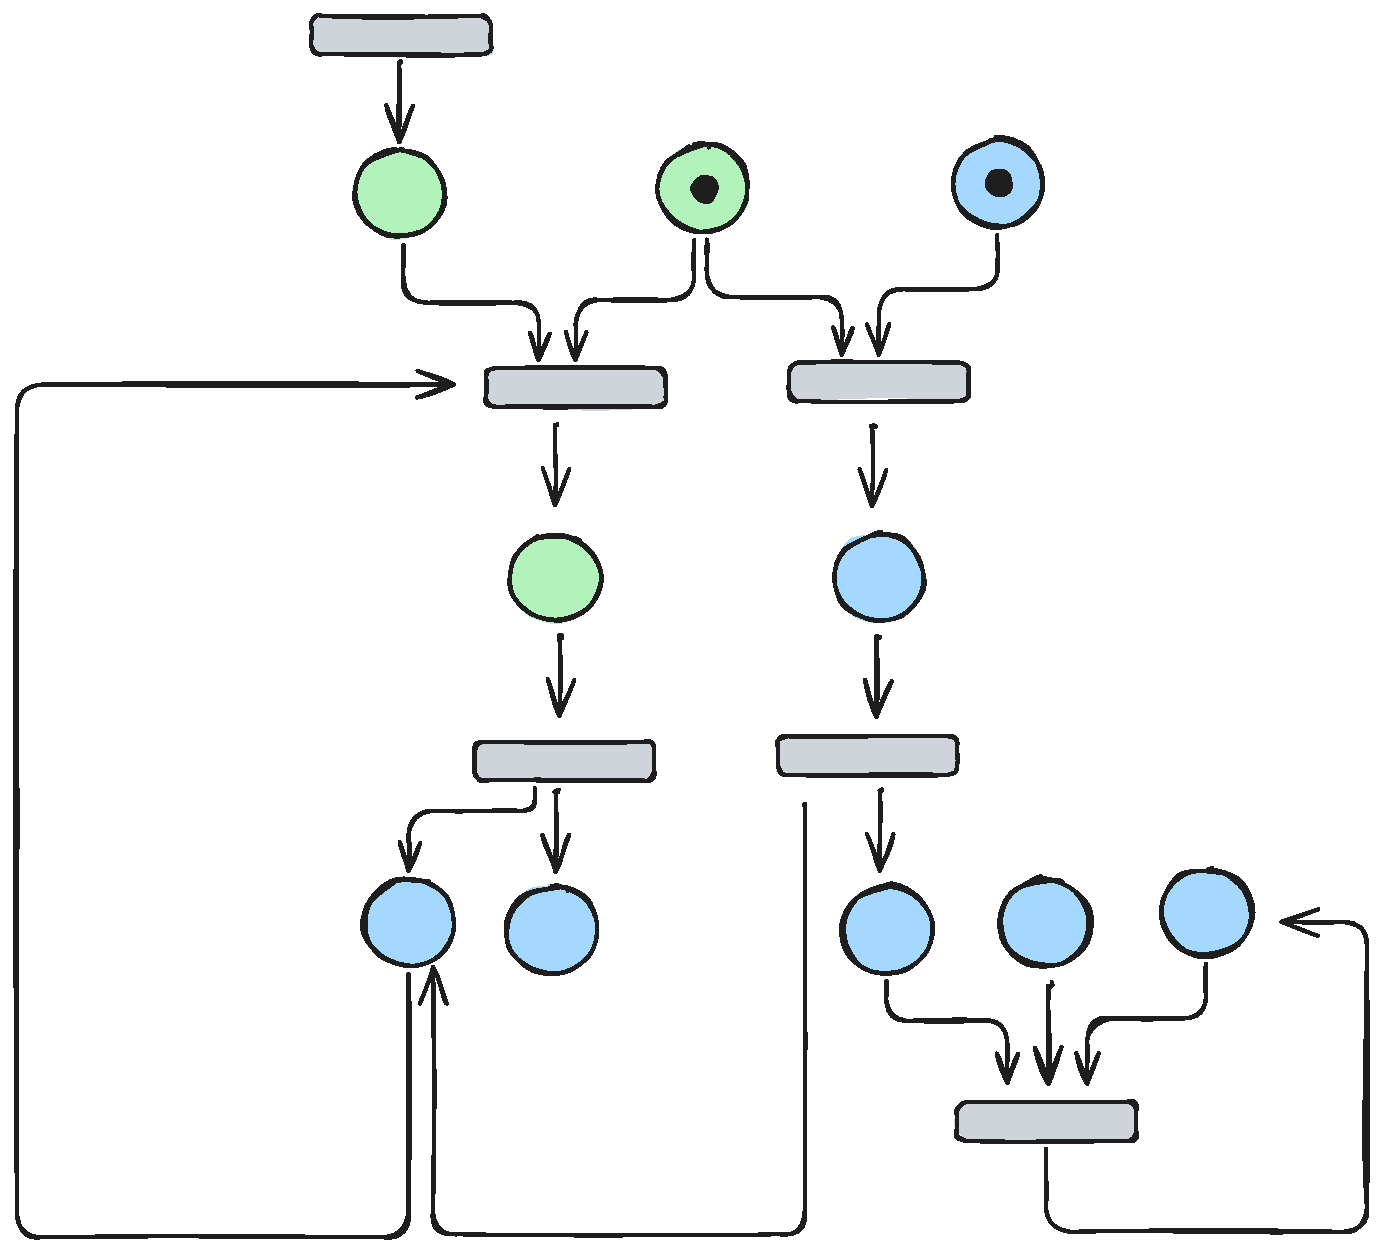
\includegraphics[width=\textwidth]{plots/bidirectional_pruning_step_a_updated.pdf}
		\caption{Step 0: initial Petri Net, before pruning.}
		\label{fig:step:a}
	\end{subfigure}\hfill
	\begin{subfigure}[b]{0.45\textwidth}
		\centering
		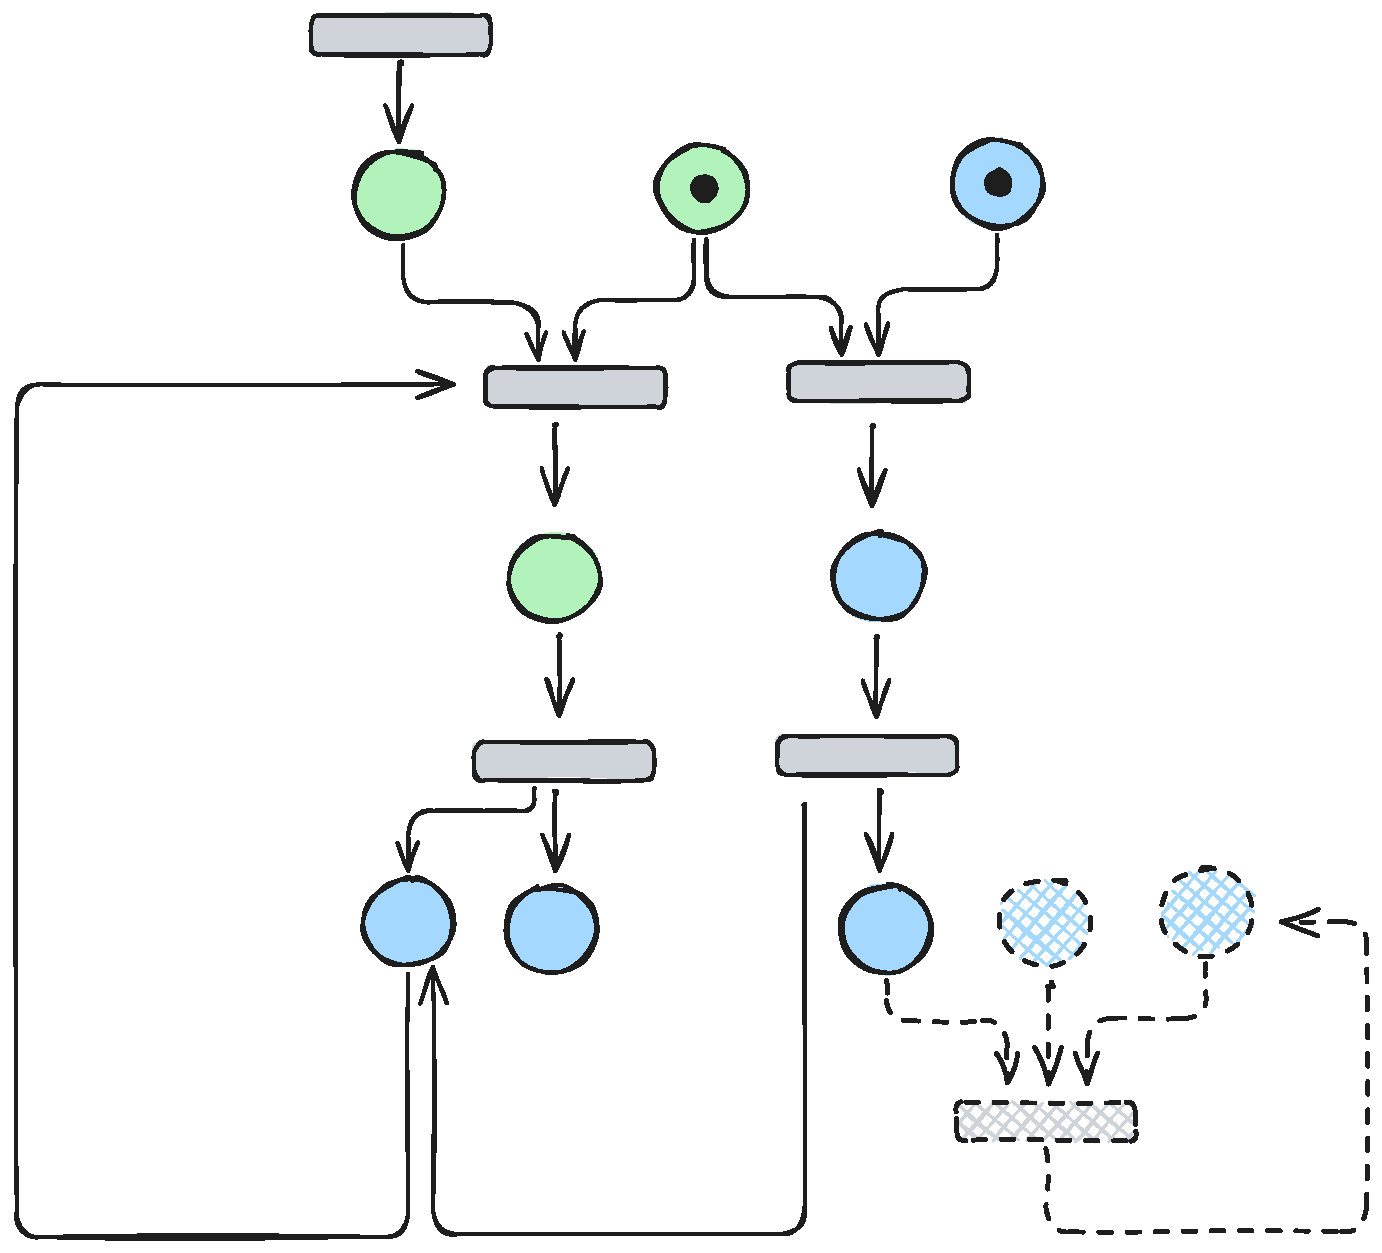
\includegraphics[width=\textwidth]{plots/bidirectional_pruning_step_b_updated.pdf}
		\caption{Step 1: first forward pass.}
		\label{fig:step:b}
	\end{subfigure}
	
	\vspace{1em}
	
	% Bottom row: (c), (d), and (e) matching (d)’s height
	\begin{subfigure}[b]{0.30\textwidth}
		\centering
		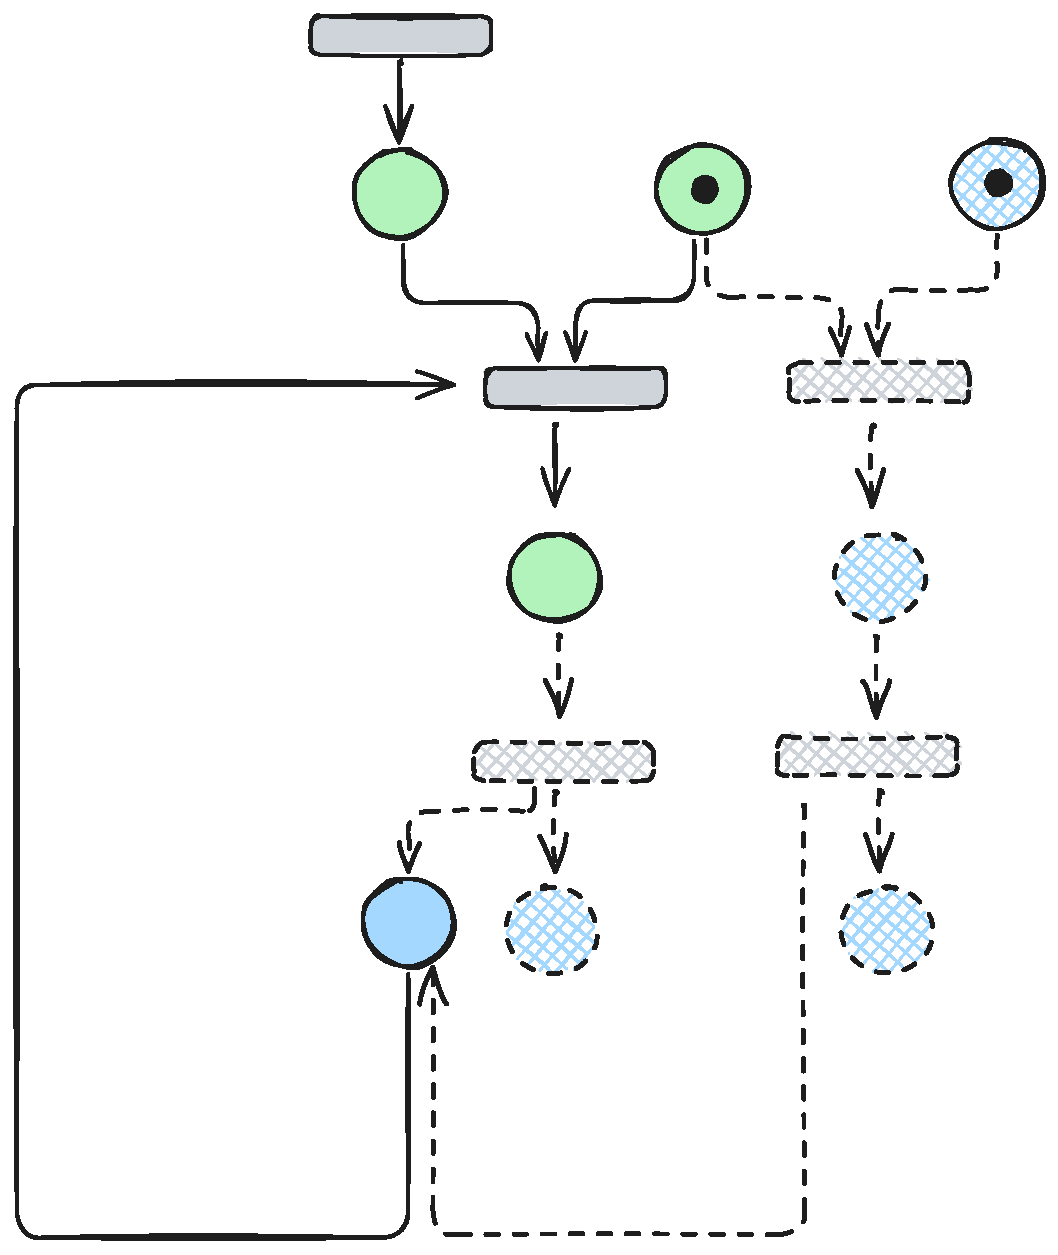
\includegraphics[width=\textwidth]{plots/bidirectional_pruning_step_c_updated.pdf}
		\caption{Step 3: first backward pass.}
		\label{fig:step:c}
	\end{subfigure}\hfill
	\begin{subfigure}[b]{0.23\textwidth}
		\centering
		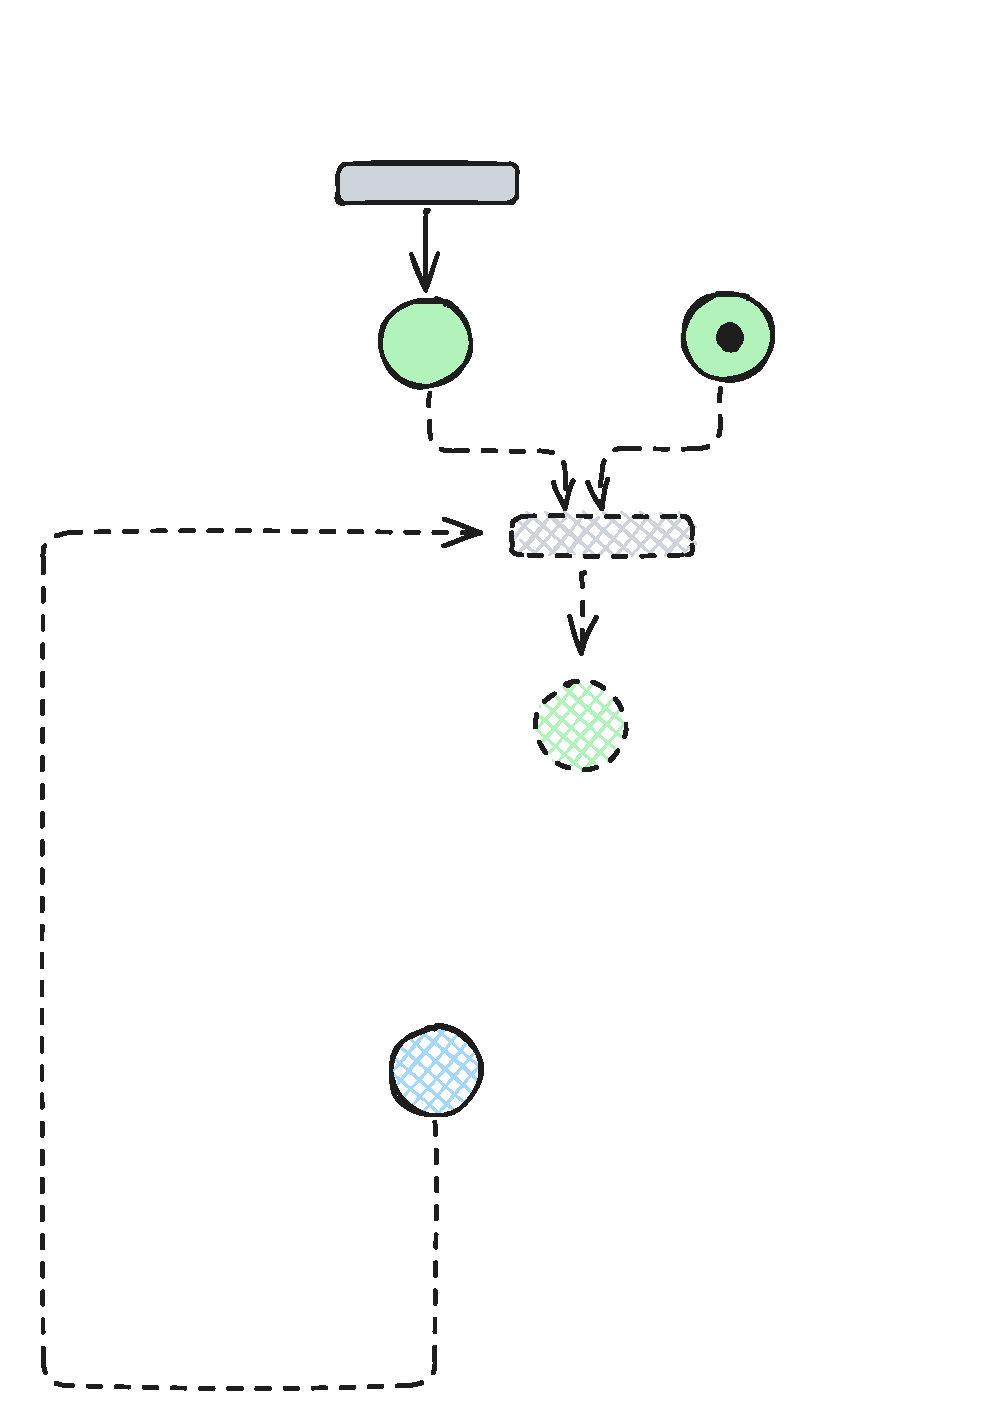
\includegraphics[width=\textwidth]{plots/bidirectional_pruning_step_d_updated_2.pdf}
		\caption{Step 4: second forward pass.}
		\label{fig:step:d}
	\end{subfigure}\hfill
	% <-- three-arg form: [vpos][total height][inner vpos]
	\begin{subfigure}[b][\subfigheight][b]{0.23\textwidth}
		\centering
		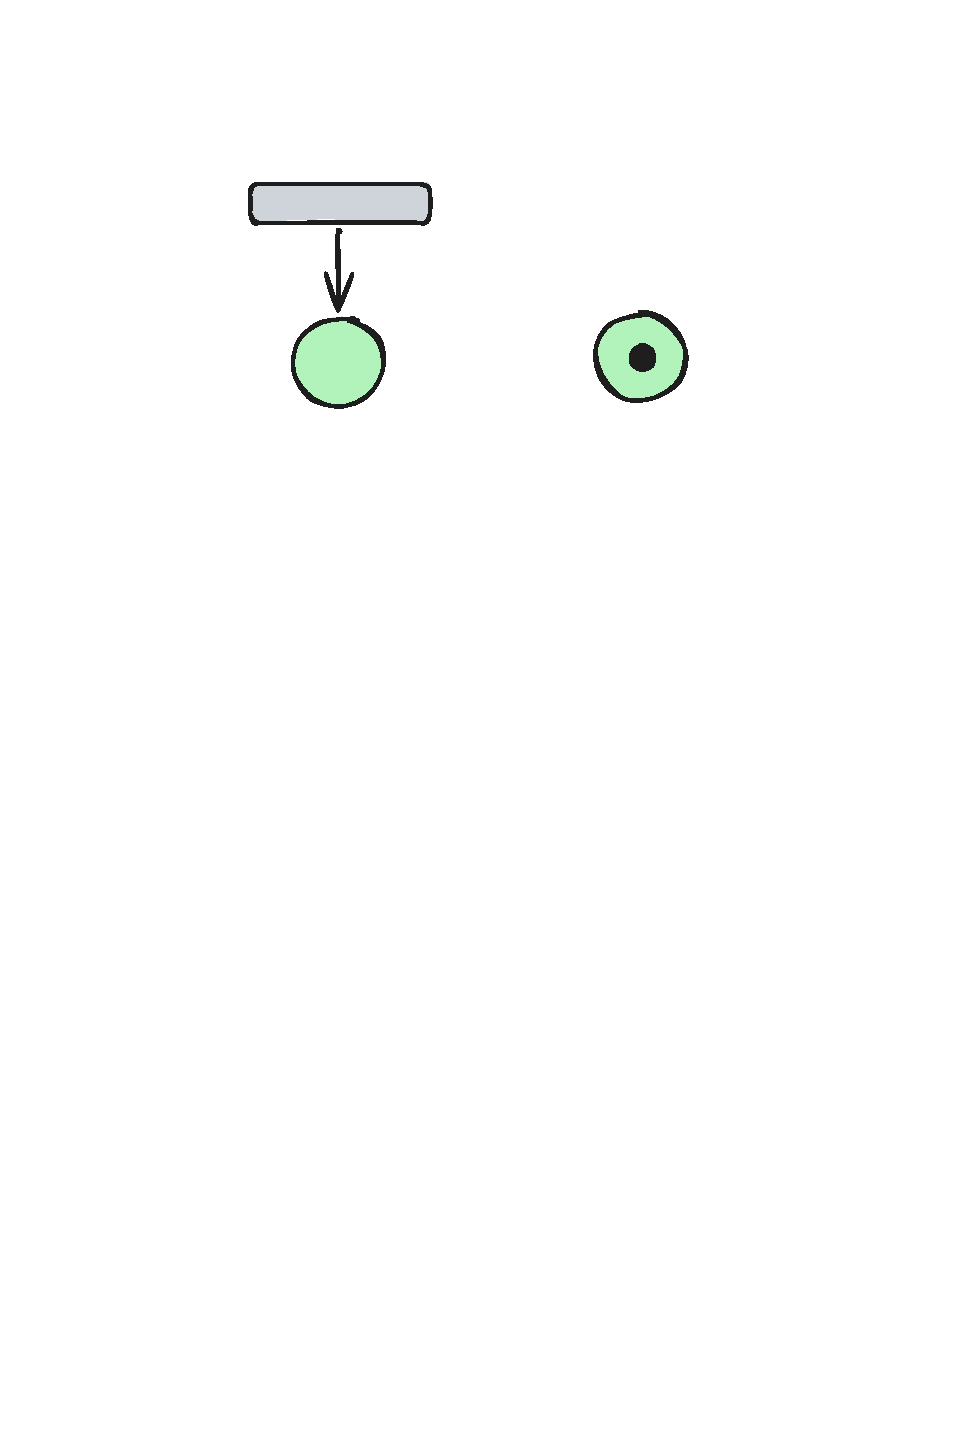
\includegraphics[width=\textwidth]{plots/bidirectional_pruning_step_e_updated_2.pdf}
		\caption{Step 6: final Petri Net.}
		\label{fig:step:e}
	\end{subfigure}
	
	\caption{A Petri net after three rounds of bidirectional pruning: two forward passes and one backward pass. Black dots represent initial token markings; green places represent places that are allowed to be reachable in our constraints (i.e., aren't fixed to zero tokens in the final marking). Dashed shapes represent places and transitions that are identified as removable in the current iteration, and will be removed after it ends.}
	\label{fig:bidirectional_pruning}
\end{figure}

%\newpage
